\section{General usage of \iLaTeX{}}

\subsection{How to setup the \iLaTeX{} extension?}
The \iLaTeX{} extension is provided as a regular extension for the \vsc editor.
It comes in the form of a single file with a \texttt{.vsix} extension.
To install the extension from this file, you should open the extensions panel by clicking the Extensions button in the Activity bar (that is normally on the left-hand side of every \vsc window). From there, you should click the icon with three dots in the top-right hand corner, select the ``Install from VSIX...'' entry, and select the \texttt{ilatex.vsix} file that was provided by the investigator.
The procedure is illustrated in \autoref{fig:install-procedure}.
Note that you can also uninstall the extension from this panel (by clicking on the gear icon next to the entry corresponding to the \iLaTeX{} extension in the list and selecting the ``Uninstall'' option).

Once the \iLaTeX{} extension in installed in \vsc, it will be automatically running in the background every time you open the editor.
You can tell the \iLaTeX{} extension is activated by checking if there is an ``i-LaTeX'' button in the status bar.
It is normally displayed in the bottom-left hand corner of every \vsc window (\autoref{subfig:status-bar-with-ilatex-button}).

When the extension is idle, the circle in the button is empty.
On the contrary, when one or more interactive \LaTeX{} documents are currently open, the circle in the button is filled, and the number of active documents is displayed between parentheses (\autoref{subfig:status-bar-buttons}).

\begin{figure}[b!]
    \centering
    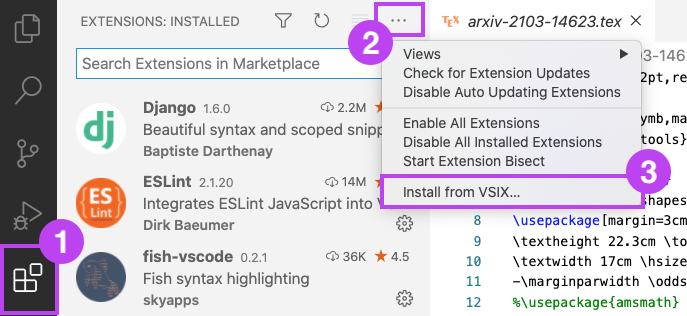
\includegraphics[width=0.8\textwidth]{img/installation-procedure.png}
    \caption{Procedure to install the \iLaTeX{} extension: \figstep{1} open the Extensions panel; \figstep{2} open the menu of the panel; \figstep{3} select the VSIX file of the extension.}
    \label{fig:install-procedure}
\end{figure}

\subsection{How to open a \LaTeX{} document with \iLaTeX{}?}
In order to compile and view a \LaTeX{} document with \iLaTeX{}, you must tell \iLaTeX{} which file is the \emph{main} file of your document (\ie the \emph{Main document} in Overleaf, the file you would compile with a command-line tool such as \texttt{pdflatex} or \texttt{latexmk}).
The simplest way to do this is to click the \iLaTeX{} button in the status bar: it will display a popup menu that contains different options to open a new \LaTeX{} document with \iLaTeX{} (\autoref{fig:open-with-ilatex-menu}).
From this menu, you can either choose ``Create from the active editor'' to use the document open in the editor panel that currently has the focus, or you can choose ``Create from file\dots'' to open a file selector.
Every option has a variant that opens the file with \iLaTeX{} but disables the interactive visualisations (the PDF will still be displayed, but there will be no IIR).

Finally, note that you can close an interactive document at any time by closing the panel that displays the PDF of that document.

\begin{figure}[h]
    \centering
    \begin{subfigure}[b]{0.6\textwidth}
        \centering
        
\includegraphics[width=0.6\textwidth]{img/vsc-status-bar-2.png}
        \caption{The left-hand side of the status bar.}
        \label{subfig:status-bar-with-ilatex-button}
    \end{subfigure}%
    \begin{subfigure}[b]{0.4\textwidth}
        \centering
        
\includegraphics[scale = 0.5]{img/ilatex-button-off.png} \qquad
        
\includegraphics[scale = 0.5]{img/ilatex-button-on.png}
        \caption{The two states of the \iLaTeX{} button.}
        \label{subfig:status-bar-buttons}
    \end{subfigure}
    \caption{The status bar of \vsc when the \iLaTeX{} extension is activated.}
    \label{fig:status-bar}
\end{figure}

\begin{figure}[h]
    \centering
    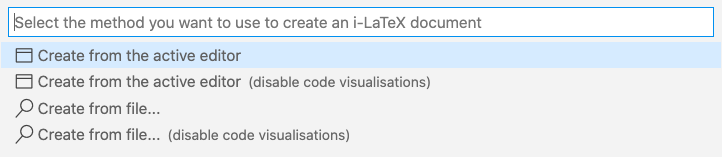
\includegraphics[width = 0.8\textwidth]{img/ilatex-menu.png}
    \caption{The popup menu that can be used to open a \LaTeX{} document with \iLaTeX{}.}
    \label{fig:open-with-ilatex-menu}
\end{figure}

\subsection{How to enable IIRs?}
\label{ssec:how-to-enable-iirs}
Every time you open a \LaTeX{} document with \iLaTeX{} and every time you save a file, \iLaTeX{} will (1) recompile the \LaTeX{} documents you opened with it and (2) attempt to locate every piece of visualisable code in your document and to create an IIR for every of them.
Visualisable code is detected by the usage of \textbf{special \LaTeX{} commands and environments} that are known to be visualisable by \iLaTeX{}.
They are covered in more details in \autoref{sec:list-of-irrs}.

In order to have access to these special commands and environments, you \textbf{must} use a special package named \texttt{ilatex}.
To do so, you must put a copy of the \texttt{ilatex.sty} file in the same directory than the main file of every \LaTeX{} document you would like to open with \iLaTeX{}, and you must include the package in the preamble of every document (\ie before the \verb|\begin{document}| command) using

\begin{lstlisting}[style=custom-latex]
\usepackage{ilatex}
\end{lstlisting}

\begin{warning}
    When you edit the code of the document, \iLaTeX{} does its best to keep track of the start and the end of every piece of visualisable code in the document.
    However, in some situations, \iLaTeX{} may be \textbf{unable to understand} the syntax of your code, or it may \textbf{loose track} of a piece of visualisable code.
    In particular, the latter is likely to happen if you edit a selection that contains text that is both within and outside the range of a visualisable piece of code.
    
    When it happens, \iLaTeX{} will show you it lost track of a piece of visualisable code by highlighting this piece of code in red.
    You have two options to fix this kind of problem:
    
    \begin{itemize}
        \item \textbf{In case of a syntax error} (\eg a curly bracket ``\verb|{|'' that has no matching closing bracket ``\verb|}|''), you can simply edit the code to fix the error, and \iLaTeX{} will remove the red highlighting as soon as the syntax becomes valid again.
        
        \item \textbf{Otherwise}, you should recompile the document to force \iLaTeX{} to re-detect all the visualisable pieces of code and re-create all IIRs.
        This can be done by clicking the message displayed above the piece of code highlighted in red, by clicking the ``Recompile'' button displayed on top of the PDF, or by saving the document.
    \end{itemize}
\end{warning}


\subsection{How to display IIRs?}

Each piece of visualisable code is normally associated with an element in the PDF (the element that was created by this piece of code).
Every such element will be \textbf{surrounded by a blue halo} in the PDF displayed by \iLaTeX{}, and you can display the IIR related to that element by clicking on it.
Depending on the position of the clicked element on your screen, the IIR will be displayed either below or above the element in the PDF---so that you can always look at the element while you use the IIR.

Some features are common to all IIRs:
\begin{itemize}%[noitemsep]
    \item You can \textbf{show the code} that is being visualised in an IIR by clicking on the title bar of the title of the visualisation (at the top of the popup). \iLaTeX{} will automatically open the file that contains the code (or give the focus to the panel where it is currently open) and scroll to it.
    \item You can \textbf{close the IIR} by either (1) clicking the button in the top-right hand corner or (2) clicking anywhere on the darkened background displayed on top of the PDF. If you modified the code of the document by interacting with the IIR, the document will automatically be \textbf{saved and recompiled} when the IIR is closed.
\end{itemize}

In some cases, the halo of one or several element may also turn grey (\autoref{subfig:grey-halo}).
A \textbf{grey halo} means that an IIR exists for this element but is \textbf{not available} at the moment.

The halo of an element will become grey if \iLaTeX{} is unable to parse the syntax of the code of this element
In addition, all halos will turn grey every time \textbf{your document is being compiled} (you cannot use an IIR while compiling), and every time \textbf{the last compilation of your document failed} (you will be notified by a popup message when it fails).
If you fix all the errors and recompile your document, the halo should eventually turn blue again.

\begin{info}
    When an IIR is displayed, you can of course interact with it, but you can also keep editing the source code of your document.
    \iLaTeX{} will automatically update the IIR to keep in synchronised with the piece of code it is associated to.
    This can be used to see how a certain change in the code affects the visualisation without having to recompile the entire document.
        
    In case you introduce a syntax error while you edit the code, the IIR will turn yellow and display an error message (\autoref{subfig:syntax-error-in-iir}).
    The content of the IIR should be restored as soon as the syntax becomes valid again.
    If an IIR is stuck in this state, try closing and reopening it.
    If it does not work, try saving the changes and recompiling the document.

\end{info}

\begin{figure}[h]
    \centering
    \begin{subfigure}[b]{0.5\textwidth}
        \centering
        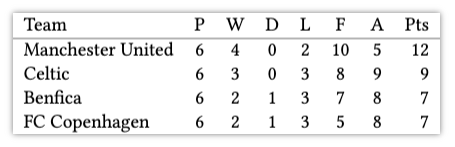
\includegraphics[width=0.8\textwidth]{img/disabled-table.png}
        \caption{A PDF element with a disabled IIR.}
        \label{subfig:grey-halo}
    \end{subfigure}%
    \begin{subfigure}[b]{0.5\textwidth}
        \centering
        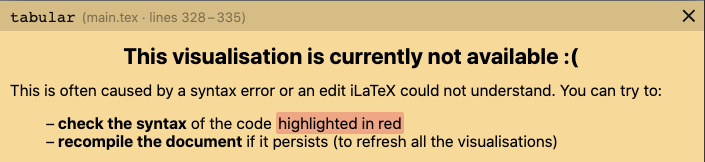
\includegraphics[width=\textwidth]{img/syntax-error-in-visualisation.png}
        \caption{An IIR displaying an error.}
        \label{subfig:syntax-error-in-iir}
    \end{subfigure}%
    \caption{(\subref{subfig:grey-halo}) When an IIR becomes disabled, the halo around the element it corresponds to in the PDF becomes grey. (\subref{subfig:syntax-error-in-iir}) If the visualisation is already displayed when it happens, it will turn yellow and display an error message.}
    \label{fig:disabled-visualisations}
\end{figure}